% TikZ / pgfplots / circuitikz gallery.
% Compile: latexmk -pdf tikz-examples.tex
% All three packages ship with TeX Live full; tectonic downloads them on demand.
\documentclass[11pt,a4paper]{article}

\usepackage[margin=2.5cm]{geometry}
\usepackage{tikz}
\usetikzlibrary{arrows.meta,positioning,shapes.geometric}
\usepackage{pgfplots}
\pgfplotsset{compat=1.18}
\usepackage{circuitikz}

\begin{document}

\section*{TikZ Examples Gallery}

\subsection*{1. Block diagram (nodes + arrows)}

\begin{center}
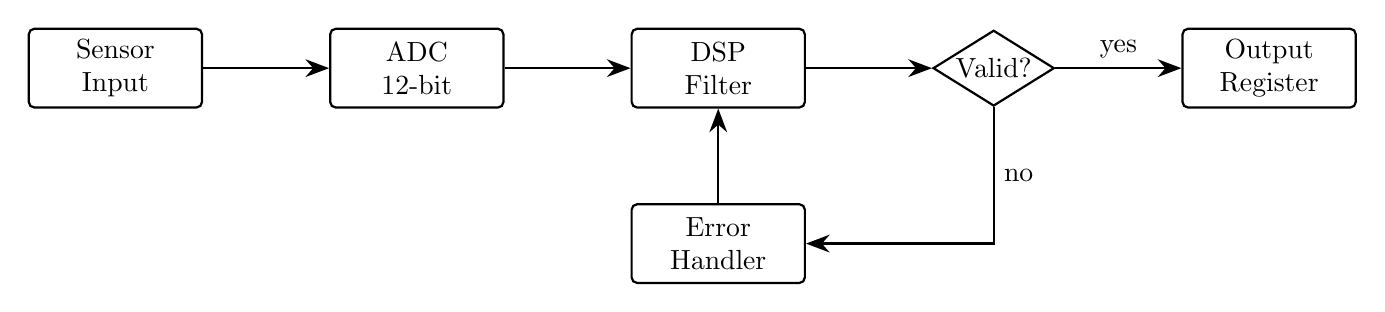
\begin{tikzpicture}[
    node distance=1.2cm and 1.6cm,
    block/.style={rectangle, draw, thick, minimum width=2.2cm,
                  minimum height=1cm, align=center, rounded corners=2pt},
    decision/.style={diamond, draw, thick, aspect=1.6, align=center,
                     inner sep=1pt},
    line/.style={-{Stealth[length=3mm]}, thick}
]
  \node[block] (input) {Sensor\\Input};
  \node[block, right=of input] (adc) {ADC\\12-bit};
  \node[block, right=of adc] (dsp) {DSP\\Filter};
  \node[decision, right=of dsp] (check) {Valid?};
  \node[block, right=of check] (out) {Output\\Register};
  \node[block, below=of dsp] (err) {Error\\Handler};

  \draw[line] (input) -- (adc);
  \draw[line] (adc) -- (dsp);
  \draw[line] (dsp) -- (check);
  \draw[line] (check) -- node[above] {yes} (out);
  \draw[line] (check) |- node[near start, right] {no} (err);
  \draw[line] (err) -- (dsp);
\end{tikzpicture}
\end{center}

\subsection*{2. Plot with pgfplots}

\begin{center}
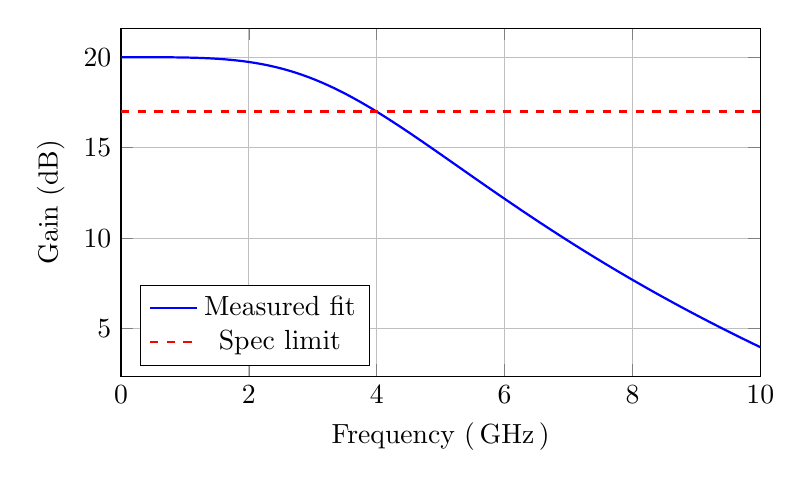
\begin{tikzpicture}
  \begin{axis}[
      width=0.8\textwidth, height=6cm,
      xlabel={Frequency (\,GHz\,)},
      ylabel={Gain (dB)},
      grid=major,
      legend pos=south west,
      xmin=0, xmax=10,
  ]
    \addplot[blue, thick, domain=0:10, samples=100]
      { 20 - 10*ln(1 + (x/4)^4)/ln(10) };
    \addlegendentry{Measured fit}

    \addplot[red, dashed, thick] coordinates {(0,17) (10,17)};
    \addlegendentry{Spec limit}
  \end{axis}
\end{tikzpicture}
\end{center}

\subsection*{3. Circuit with circuitikz}

\begin{center}
\begin{circuitikz}[american]
  \draw (0,0)
    to[V, v=$V_s$] (0,3)          % source
    to[R, l=$R_1$, i=$i$] (3,3)   % series resistor
    to[C, l=$C_1$] (3,0)          % capacitor to ground
    -- (0,0);
  \draw (3,3)
    to[short] (5,3)
    to[R, l=$R_L$] (5,0)
    to[short] (3,0);
  \draw (1.5,0) node[ground]{};
\end{circuitikz}
\end{center}

A first-order RC low-pass driving a load $R_L$; cutoff at
$f_c = 1/(2\pi R_1 C_1)$.

\end{document}
